\documentclass[12pt, titlepage]{article}

\usepackage{fullpage}
\usepackage[round]{natbib}
\usepackage{multirow}
\usepackage{booktabs}
\usepackage{tabularx}
\usepackage{graphicx}
\usepackage{float}
\usepackage{hyperref}
\hypersetup{
    colorlinks,
    citecolor=blue,
    filecolor=black,
    linkcolor=red,
    urlcolor=blue
}

%% Comments

\usepackage{color}

\newif\ifcomments\commentstrue %displays comments
%\newif\ifcomments\commentsfalse %so that comments do not display

\ifcomments
\newcommand{\authornote}[3]{\textcolor{#1}{[#3 ---#2]}}
\newcommand{\todo}[1]{\textcolor{red}{[TODO: #1]}}
\else
\newcommand{\authornote}[3]{}
\newcommand{\todo}[1]{}
\fi

\newcommand{\wss}[1]{\authornote{blue}{SS}{#1}} 
\newcommand{\plt}[1]{\authornote{magenta}{TPLT}{#1}} %For explanation of the template
\newcommand{\an}[1]{\authornote{cyan}{Author}{#1}}

%% Common Parts

\newcommand{\progname}{Software Engineering} % PUT YOUR PROGRAM NAME HERE
\newcommand{\authname}{Team 17, Track a Trace
\\ Zabrain Ali
\\ Linqi Jiang
\\ Jasper Leung
\\ Mike Li 
\\ Mengtong Shi
\\ Hongzhao Tan
} % AUTHOR NAMES                  

\usepackage{hyperref}
    \hypersetup{colorlinks=true, linkcolor=blue, citecolor=blue, filecolor=blue,
                urlcolor=blue, unicode=false}
    \urlstyle{same}
                                


\newcounter{acnum}
\newcommand{\actheacnum}{AC\theacnum}
\newcommand{\acref}[1]{AC\ref{#1}}

\newcounter{ucnum}
\newcommand{\uctheucnum}{UC\theucnum}
\newcommand{\uref}[1]{UC\ref{#1}}

\newcounter{mnum}
\newcommand{\mthemnum}{M\themnum}
\newcommand{\mref}[1]{M\ref{#1}}

\begin{document}

\title{Module Guide for \progname{}} 
\author{\authname}
\date{January 18, 2023}

\maketitle

\pagenumbering{roman}

\section{Revision History}

\begin{tabularx}{\textwidth}{p{3cm}p{2cm}X}
\toprule {\bf Date} & {\bf Version} & {\bf Notes}\\
\midrule
January 13, 2023 & 1.0 & Edited Abbreviations and Acronyms, Introduction, Anticipated and Unlikely Changes, Module Hierarchy\\
January 14, 2023 & 1.1 & Edited Connection Between Requirements and Design and Module Decomposition\\
January 18, 2023 & 1.2 & Edited Traceability Matrix and Use Hierarchy Between Modules\\
\bottomrule
\end{tabularx}

\newpage

\section{Reference Material}

This section records information for easy reference.

\subsection{Abbreviations and Acronyms}

\renewcommand{\arraystretch}{1.2}
\begin{tabular}{l l} 
  \toprule		
  \textbf{symbol} & \textbf{description}\\
  \midrule 
  AC & Anticipated Change\\
  DAG & Directed Acyclic Graph \\
  M & Module \\
  MG & Module Guide \\
  OS & Operating System \\
  R & Requirement\\
  SC & Scientific Computing \\
  SRS & Software Requirements Specification\\
  \progname & Explanation of program name\\
  UC & Unlikely Change \\
  OSM & OpenStreetMap \\
  2D & two-dimensional\\
  GIS & geographic information system\\
  SHP & shapefile: a geospatial vector data format for GIS software\\
%   \wss{etc.} & \wss{...}\\
  \bottomrule
\end{tabular}\\

\newpage

\tableofcontents

\listoftables

\listoffigures

\newpage

\pagenumbering{arabic}

\section{Introduction}

Decomposing a system into modules is a commonly accepted approach to developing
software.  A module is a work assignment for a programmer or programming
team~\citep{ParnasEtAl1984}.  We advocate a decomposition
based on the principle of information hiding~\citep{Parnas1972a}.  This
principle supports design for change, because the ``secrets'' that each module
hides represent likely future changes.  Design for change is valuable in SC,
where modifications are frequent, especially during initial development as the
solution space is explored.  

Our design follows the rules layed out by \citet{ParnasEtAl1984}, as follows:
\begin{itemize}
\item System details that are likely to change independently should be the
  secrets of separate modules.
\item Each data structure is implemented in only one module.
\item Any other program that requires information stored in a module's data
  structures must obtain it by calling access programs belonging to that module.
\end{itemize}

After completing the first stage of the design, the Software Requirements
Specification (SRS), the Module Guide (MG) is developed~\citep{ParnasEtAl1984}. The MG
specifies the modular structure of the system and is intended to allow both
designers and maintainers to easily identify the parts of the software.  The
potential readers of this document are as follows:

\begin{itemize}
\item New project members: This document can be a guide for a new project member
  to easily understand the overall structure and quickly find the
  relevant modules they are searching for.
\item Maintainers: The hierarchical structure of the module guide improves the
  maintainers' understanding when they need to make changes to the system. It is
  important for a maintainer to update the relevant sections of the document
  after changes have been made.
\item Designers: Once the module guide has been written, it can be used to
  check for consistency, feasibility, and flexibility. Designers can verify the
  system in various ways, such as consistency among modules, feasibility of the
  decomposition, and flexibility of the design.
\end{itemize}

The rest of the document is organized as follows. Section
\ref{SecChange} lists the anticipated and unlikely changes of the software
requirements. Section \ref{SecMH} summarizes the module decomposition that
was constructed according to the likely changes. Section \ref{SecConnection}
specifies the connections between the software requirements and the
modules. Section \ref{SecMD} gives a detailed description of the
modules. Section \ref{SecTM} includes two traceability matrices. One checks
the completeness of the design against the requirements provided in the SRS. The
other shows the relation between anticipated changes and the modules. Section
\ref{SecUse} describes the use relation between modules.

\section{Anticipated and Unlikely Changes} \label{SecChange}

This section lists possible changes to the system. According to the likeliness
of the change, the possible changes are classified into two
categories. Anticipated changes are listed in Section \ref{SecAchange}, and
unlikely changes are listed in Section \ref{SecUchange}.

\subsection{Anticipated Changes} \label{SecAchange}

\begin{description}
\item[\refstepcounter{acnum} \actheacnum \label{acHardware}:] The specific
  hardware on which the software is running.
\item[\refstepcounter{acnum} \actheacnum \label{acRCSG}:]  The implementation for the methods for generating route choice set.
\item[\refstepcounter{acnum} \actheacnum \label{acRCAVG}:]  The implementation for the methods for generating route choice analysis variable.
\item[\refstepcounter{acnum} \actheacnum \label{acGOAM}:] The specific algorithms that are used for geometric object analysis and manipulation.
\item[\refstepcounter{acnum} \actheacnum \label{acNA}:] The specific algorithms that are used for network analysis.
\end{description}

\subsection{Unlikely Changes} \label{SecUchange}

\begin{description}
\item[\refstepcounter{ucnum} \uctheucnum \label{ucGPD}:] An unlikely change for the module design is the implementation being designed around the open-source free library GeoPandas
\item [\refstepcounter{ucnum} \uctheucnum \label{ucGDF}:] An unlikely change for the module design is building the modules based on the GeoDataFrame object which is a panadas.DataFrame that has a column with geometry
\item [\refstepcounter{ucnum} \uctheucnum \label{ucP}:] An unlikely change for the module design is to use the geojsonio package to transfer the geopandas dataframe to geojson format which will then be converted to a json string to display the GPS points
\item [\refstepcounter{ucnum} \uctheucnum \label{ucOSMNDR}:] An unlikely change for the module design is use pyrosm to create the GeoDataFrame for driving network and buildings from OpenStreetMap PBF files
\end{description}

\section{Module Hierarchy} \label{SecMH}

This section provides an overview of the module design. Modules are summarized
in a hierarchy decomposed by secrets in Table \ref{TblMH}. The modules listed
below, which are leaves in the hierarchy tree, are the modules that will
actually be implemented.

\begin{description}
\item [\refstepcounter{mnum} \mthemnum \label{mHH}:] Hardware-Hiding Module
\item [\refstepcounter{mnum} \mthemnum \label{mGP}:] GPS Data Preprocessing Module 
\item [\refstepcounter{mnum} \mthemnum \label{mMD}:] GPS Data Mode Detection Module 
\item [\refstepcounter{mnum} \mthemnum \label{mTSALE}:] Trip Segments and Activity Locations Extraction Module
\item [\refstepcounter{mnum} \mthemnum \label{mRCS}:] Route Choice Set Generator Module
\item [\refstepcounter{mnum} \mthemnum \label{mRCAV}:] Route Choice Analysis Variables Generator Module
\item [\refstepcounter{mnum} \mthemnum \label{mALI}:] Activity Locations Identification Module
\item [\refstepcounter{mnum} \mthemnum \label{mMF}:] Main Function Module
\item [\refstepcounter{mnum} \mthemnum \label{mDFDS}:] Dataframe Data Structure Module
\item [\refstepcounter{mnum} \mthemnum \label{mGDFDS}:] GeoDataframe Data Structure Module
\item [\refstepcounter{mnum} \mthemnum \label{mGOAM}:] Geometric Object Analysis and Manipulation Module
\item [\refstepcounter{mnum} \mthemnum \label{mNA}:] Network Analysis Module
\item [\refstepcounter{mnum} \mthemnum \label{mOSMNDR}:] OSM Network Dataset Reader Module
\item [\refstepcounter{mnum} \mthemnum \label{mP}:] Plotting Module
\end{description}


\begin{table}[h!]
\centering
\begin{tabular}{p{0.3\textwidth} p{0.6\textwidth}}
\toprule
\textbf{Level 1} & \textbf{Level 2}\\
\midrule

{Hardware-Hiding Module} & ~ \\
\midrule

\multirow{7}{0.3\textwidth}{Behaviour-Hiding Module}
& GPS Data Preprocessing Module\\
& GPS Data Mode Detection Module \\
& Trip Segments and Activity Locations Extraction Module\\
& Route Choice Set Generator Module\\
& Route Choice Analysis Variables Generator Module\\
& Activity Locations Identification Module\\
& Main Function Module\\ 
\midrule

\multirow{3}{0.3\textwidth}{Software Decision Module}
& Dataframe Data Structure Module\\
& GeoDataframe Data Structure Module\\
& Geometric Object Analysis and Manipulation Module\\
& Network Analysis Module\\
& OSM Network Dataset Reader Module\\
& Plotting Module\\
\bottomrule

\end{tabular}
\caption{Module Hierarchy}
\label{TblMH}
\end{table}

\section{Connection Between Requirements and Design} \label{SecConnection}

The design of the system is intended to satisfy the requirements developed in
the \href{https://github.com/paezha/PyERT-BLACK/blob/main/docs/SRS/SRS.pdf}{SRS} \citep{SRS}. In this stage, the system is decomposed into modules. The connection
between requirements and modules is listed in Table~\ref{TblRT}.

\section{Module Decomposition} \label{SecMD}

Modules are decomposed according to the principle of ``information hiding''
proposed by \citet{ParnasEtAl1984}. The \emph{Secrets} field in a module
decomposition is a brief statement of the design decision hidden by the
module. The \emph{Services} field specifies \emph{what} the module will do
without documenting \emph{how} to do it. For each module, a suggestion for the
implementing software is given under the \emph{Implemented By} title. If the
entry is \emph{OS}, this means that the module is provided by the operating
system or by standard programming language libraries.  \emph{\progname{}} means the
module will be implemented by the \progname{} software.

Only the leaf modules in the hierarchy have to be implemented. If a dash
(\emph{--}) is shown, this means that the module is not a leaf and will not have
to be implemented.

\subsection{Hardware Hiding Modules (\mref{mHH})}

\begin{description}
\item[Secrets:]The data structure and algorithm used to implement the virtual
  hardware.
\item[Services:]Serves as a virtual hardware used by the rest of the
  system. This module provides the interface between the hardware and the
  software. So, the system can use it to display outputs or to accept inputs.
\item[Implemented By:] OS
\end{description}

\subsection{Behaviour-Hiding Module}

\begin{description}
\item[Secrets:]The contents of the required behaviours.
\item[Services:]Includes programs that provide externally visible behaviour of
  the system as specified in the software requirements specification (\href{https://github.com/paezha/PyERT-BLACK/blob/main/docs/SRS/SRS.pdf}{SRS} \citep{SRS})
  documents. This module serves as a communication layer between the
  hardware-hiding module and the software decision module. The programs in this
  module will need to change if there are changes in the \href{https://github.com/paezha/PyERT-BLACK/blob/main/docs/SRS/SRS.pdf}{SRS} \citep{SRS}.
\item[Implemented By:] --
\end{description}

\subsubsection{GPS Data Preprocessing Module (\mref{mGP})}

\begin{description}
\item[Secrets:]The algorithms and functions for prerpocessing the raw GPS data.
\item[Services:]Removes invalid data from the raw GPS data from user's input.
\item[Implemented By:] PyERT
\item[Type of Module:] Library
\end{description}

\subsubsection{GPS Data Mode Detection Module (\mref{mMD})}
\begin{description}
\item[Secrets:]The algorithms and functions detecting the modes(e.g. drive, walk, stop) of GPS data.
\item[Services:]Classifies the valid GPS data into travel or stop episodes.
\item[Implemented By:] PyERT
\item[Type of Module:] Library
\end{description}

\subsubsection{Trip Segments and Activity Locations Extraction Module (\mref{mTSALE})}

\begin{description}
\item[Secrets:]The algorithms and functions for extracting trip segments and activity locations from GPS data
\item[Services:]Extracts trip segments(GPS points in travel episodes generated by \mref{mMD}) and activity locations (GPS points in the stop episodes generated by \mref{mMD}).
\item[Implemented By:] PyERT
\item[Type of Module:] Library
\end{description}

\subsubsection{Route Choice Set Generator Module (\mref{mRCS})}

\begin{description}
\item[Secrets:]The algorithms and functions for generating route choice sets from given trip segments.
\item[Services:]Generates route choice sets with the trip segments extracted by \mref{mTSALE} and transportation network dataset from user's input.
\item[Implemented By:] PyERT
\item[Type of Module:] Library
\end{description}

\subsubsection{Route Choice Analysis Variables Generator Module (\mref{mRCAV})}

\begin{description}
\item[Secrets:]The algorithms and functions for generating route choice analysis variables from given route choice.
\item[Services:]Generates route choice analysis variables including the number of each type of turns, the length of route by meters, the name of street for the longest leg and the length of the longest leg by meters, for the route choice generated by \mref{mRCS}, with the data of the route choice and the transportation network dataset from user's input.
\item[Implemented By:] PyERT
\item[Type of Module:] Library
\end{description}

\subsubsection{Activity Locations Identification Module (\mref{mALI})}

\begin{description}
\item[Secrets:]The algorithms and functions for appending information for extracted activity locations.
\item[Services:]Appends information for activity locations extracted by \mref{mTSALE}, if such information has been provided by the transportation network dataset from user's input.
\item[Implemented By:] PyERT
\item[Type of Module:] Library
\end{description}

\subsubsection{Main Function Module (\mref{mMF})}

\begin{description}
\item[Secrets:] The function for coordinating the running of the system.
\item[Services:] Provides the main function of the system.
\item[Implemented By:] PyERT
\end{description}


\subsection{Software Decision Module}

\begin{description}
\item[Secrets:] The design decision based on mathematical theorems, physical
  facts, or programming considerations. The secrets of this module are
  \emph{not} described in the \href{https://github.com/paezha/PyERT-BLACK/blob/main/docs/SRS/SRS.pdf}{SRS} \citep{SRS}.
\item[Services:] Includes data structure and algorithms used in the system that
  do not provide direct interaction with the user. 
  % Changes in these modules are more likely to be motivated by a desire to
  % improve performance than by externally imposed changes.
\item[Implemented By:] --
\end{description}

\subsubsection{Dataframe Data Structure Module (\mref{mDFDS})}

\begin{description}
\item[Secrets:]The data structure for a Pandas Dataframe data type.
\item[Services:] Provides 2D array(or can be seen as a table with rows and columns where values on the same column are of the same data type) manipulation, including building a 2D array, access or change the value of a specific row, column or entry, etc.
\item[Implemented By:] Pandas
\end{description}

\subsubsection{GeoDataframe Data Structure Module (\mref{mGDFDS})}

\begin{description}
\item[Secrets:]The data structure for a GeoPandas GeoDataframe data type, which is a type of specialized Pandas Dataframe with a 'geometry' column that contains geometric objects of types POINT, LINESTRING, MULTILINGSTRING, POLYGON, or etc.
\item[Services:] Provides the 2D array manipulations that are provided by Pandas Dataframe, simple methods that can be used to manipulate geometric objects, methods to read and generate SHP files, methods to convert GeoDataframe to JSON string, etc.
\item[Implemented By:] GeoPandas
\end{description}

\subsubsection{Geometric Object Analysis and Manipulation Module (\mref{mGOAM})}

\begin{description}
\item[Secrets:]The algorithms to manipulate and analyze geometric objects (e.g. POINT, LINGSTRING, MULTILINESTRING, POLYGON, etc.). It is part of the Geopandas package (see \mref{mGDFDS}), but also can be imported and used separately.
\item[Services:] Provides methods to manipulate and analyze geometric objects, such as accessing the coordinates of a geometric object, calculating the distance between two geometric objects, etc..
\item[Implemented By:] Shapely
\end{description}

\subsubsection{Network Analysis Module (\mref{mNA})}

\begin{description}
\item[Secrets:] The algorithms and functions to analyze transportation network dataset. See related \href{https://geoffboeing.com/publications/osmnx-complex-street-networks/}{journal article} \citep{OSMnxArticle} for details. 
\item[Services:] Provides methods to analyze transportation network dataset, such as accessing the coordinates of a streets and building, finding the shortest route on transportation network between two points given their coordinates, etc..
\item[Implemented By:] OSMnx
\end{description}

\subsubsection{OSM Network Dataset Reader Module (\mref{mOSMNDR})}

\begin{description}
\item[Secrets:]The algorithm to read network dataset from OSM in Protocolbuffer Binary (.pbf) format.
\item[Services:] Provides methods to extract transportation network data, buildings' information data or etc, from network dataset from OSM in Protocolbuffer Binary (.pbf) format.
\item[Implemented By:] pyrosm
\end{description}

\subsubsection{Plotting Module (\mref{mP})}

\begin{description}
\item[Secrets:]The algorithms for visualizing data of GeoJSON format.
\item[Services:] Provides methods to visualize GeoJSON data on geojson.io.
\item[Implemented By:] geojsonio
\end{description}

\section{Traceability Matrix} \label{SecTM}

This section shows two traceability matrices: between the modules and the
requirements and between the modules and the anticipated changes. See detail description for the requirements of the system in \href{https://github.com/paezha/PyERT-BLACK/blob/main/docs/SRS/SRS.pdf}{SRS} \citep{SRS}.

% the table should use mref, the requirements should be named, use something
% like fref
\begin{table}[H]
\centering
\begin{tabular}{p{0.2\textwidth} p{0.6\textwidth}}
\toprule
\textbf{Req.} & \textbf{Modules}\\
\midrule
Req \#1 & \mref{mHH}, \mref{mMF}, \mref{mDFDS}, \mref{mGDFDS}\\
Req \#2 & \mref{mGP}, \mref{mDFDS}\\
Req \#3 & \mref{mGP}, \mref{mDFDS}\\
Req \#4 & \mref{mMD}, \mref{mDFDS}\\
Req \#5 & \mref{mMD}, \mref{mDFDS}\\
Req \#6 & \mref{mTSALE}, \mref{mDFDS}, \mref{mGDFDS}\\
Req \#7 & \mref{mTSALE}, \mref{mDFDS}, \mref{mGDFDS}\\
Req \#8 & \mref{mHH}, \mref{mMF},  \mref{mRCS}, \mref{mGDFDS}, \mref{mGOAM}, \mref{mNA}, \mref{mOSMNDR}\\
Req \#9 & \mref{mHH}, \mref{mMF},  \mref{mALI}, \mref{mGDFDS}, \mref{mOSMNDR}\\
Req \#10 & \mref{mHH}, \mref{mMF}\\
Req \#11 & \mref{mMD}, \mref{mDFDS}\\
Req \#12 & \mref{mHH}, \mref{mMF},  \mref{mRCAV}, \mref{mGDFDS}, \mref{mGOAM}, \mref{mNA}, \mref{mOSMNDR}\\
LF1 & \mref{mHH}, \mref{mMF}\\
LF2 & \mref{mHH}, \mref{mMF}\\
UH1 & \mref{mHH}, \mref{mMF}, \mref{mGP}, \mref{mMD}, \mref{mTSALE}, \mref{mRCS}, \mref{mRCAV}, \mref{mALI}\\
UH2 & \mref{mHH}, \mref{mMF}\\
UH3 & \mref{mHH}, \mref{mMF}, \mref{mGP}, \mref{mMD}, \mref{mTSALE}, \mref{mRCS}, \mref{mRCAV}, \mref{mALI}\\
PR1 & \mref{mHH}, \mref{mMF}\\
PR2 & \mref{mHH}, \mref{mMF}\\
PR3 & \mref{mDFDS}, \mref{mGDFDS}, \mref{mGOAM}, \mref{mNA}, \mref{mOSMNDR}, \mref{mP}\\
OE1 & \mref{mHH}, \mref{mMF}, \mref{mGP}, \mref{mMD}, \mref{mTSALE}, \mref{mRCS}, \mref{mRCAV}, \mref{mALI}, \mref{mDFDS}, \mref{mGDFDS}, \mref{mGOAM}, \mref{mNA}, \mref{mOSMNDR}, \mref{mP}\\
OE2 & \mref{mDFDS}, \mref{mGDFDS}, \mref{mGOAM}, \mref{mNA}, \mref{mOSMNDR}, \mref{mP}\\
OE3 & \mref{mDFDS}, \mref{mGDFDS}, \mref{mGOAM}, \mref{mNA}, \mref{mOSMNDR}, \mref{mP}\\
MS1 & \mref{mMF}, \mref{mGP}, \mref{mMD}, \mref{mTSALE}, \mref{mRCS}, \mref{mRCAV}, \mref{mALI}\\
MS3 & \mref{mHH}, \mref{mMF}, \mref{mGP}, \mref{mMD},  \mref{mTSALE}, \mref{mRCS}, \mref{mRCAV}, \mref{mALI}\\
SR1 & \mref{mMF}, \mref{mGP}, \mref{mMD},  \mref{mTSALE}, \mref{mRCS}, \mref{mRCAV}, \mref{mALI}, \mref{mDFDS}, \mref{mGDFDS}, \mref{mGOAM}, \mref{mNA}, \mref{mOSMNDR}, \mref{mP}\\
SR2 & \mref{mMF}, \mref{mGP}, \mref{mMD},  \mref{mTSALE}, \mref{mRCS}, \mref{mRCAV}, \mref{mALI}, \mref{mDFDS}, \mref{mGDFDS}, \mref{mGOAM}, \mref{mNA}, \mref{mOSMNDR}, \mref{mP}\\
SR3 & \mref{mMF}, \mref{mGP}, \mref{mMD}, \mref{mTSALE}, \mref{mRCS}, \mref{mRCAV}, \mref{mALI}\\
LR1 & \mref{mDFDS}, \mref{mGDFDS}, \mref{mGOAM}, \mref{mNA}, \mref{mOSMNDR}, \mref{mP}\\



\bottomrule
\end{tabular}
\caption{Trace Between Requirements and Modules}
\label{TblRT}
\end{table}

\begin{table}[H]
\centering
\begin{tabular}{p{0.2\textwidth} p{0.6\textwidth}}
\toprule
\textbf{AC} & \textbf{Modules}\\
\midrule
\acref{acHardware} & \mref{mHH}\\
\acref{acRCSG} & \mref{mRCS}\\
\acref{acRCAVG} & \mref{mRCAV}\\
\acref{acGOAM} & \mref{mGOAM}\\
\acref{acNA} & \mref{mNA}\\
\bottomrule
\end{tabular}
\caption{Trace Between Anticipated Changes and Modules}
\label{TblACT}
\end{table}

\section{Use Hierarchy Between Modules} \label{SecUse}

In this section, the uses hierarchy between modules is
provided. \citet{Parnas1978} said of two programs A and B that A {\em uses} B if
correct execution of B may be necessary for A to complete the task described in
its specification. That is, A {\em uses} B if there exist situations in which
the correct functioning of A depends upon the availability of a correct
implementation of B.  Figure \ref{FigUH} illustrates the use relation between
the modules. It can be seen that the graph is a directed acyclic graph
(DAG). Each level of the hierarchy offers a testable and usable subset of the
system, and modules in the higher level of the hierarchy are essentially simpler
because they use modules from the lower levels.

\begin{figure}[H]
\centering
%\includegraphics[width=0.7\textwidth]{UsesHierarchy.png}
 \centering
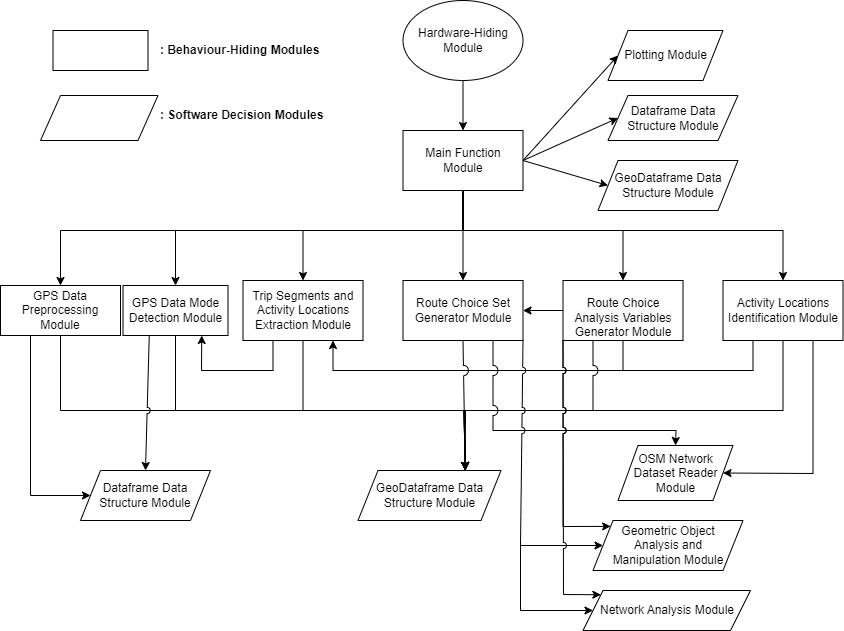
\includegraphics[scale=0.60]{UseHierarchy.png}
\caption{\bf Use Hierarchy Diagram}
\end{figure}

%\section*{References}
\newpage
\bibliographystyle {plainnat}
% \bibliography{../../../refs/References}
\bibliography{MG}

\newpage{}

\end{document}